% Figure 1: centered reliability coordinates and their logit-scale mean.
% Native Computer Modern mathematics matches the main manuscript.
% Ordinary text uses vendored Source Sans 3; native CM mathematics is unchanged.
% Build: python3 fig_src/build_fig1.py (from the manuscript directory).
\documentclass[12pt,tikz,border=0pt]{standalone}
\usepackage[no-math]{fontspec}
\usepackage{amsmath,amssymb}
\setmainfont{SourceSans3-Regular.otf}[Path=fig_src/fonts/,BoldFont=SourceSans3-Bold.otf]
\setsansfont{SourceSans3-Regular.otf}[Path=fig_src/fonts/,BoldFont=SourceSans3-Bold.otf]
\usetikzlibrary{arrows.meta}
\definecolor{okBlue}{RGB}{0,114,178}
\definecolor{okVerm}{RGB}{213,94,0}
\definecolor{ink}{RGB}{26,26,26}
\definecolor{inkGrey}{RGB}{102,102,102}
\definecolor{boxGrey}{RGB}{140,140,140}
\definecolor{boxBlue}{RGB}{239,245,250}
\begin{document}
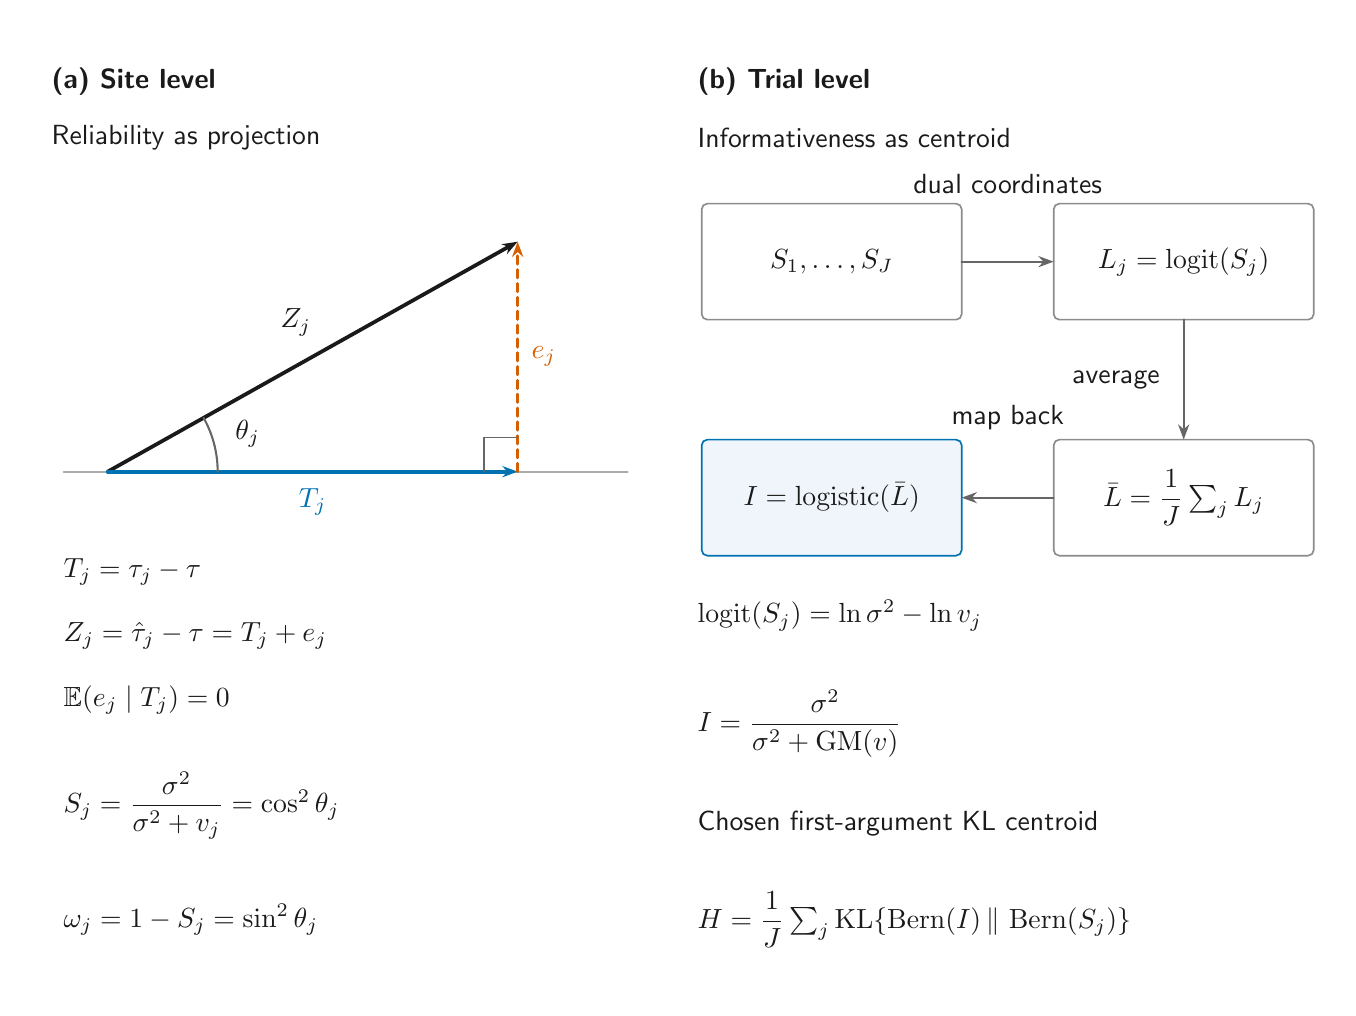
\begin{tikzpicture}[
  x=1in,y=1in,draw=ink,text=ink,line cap=round,line join=round,
  >={Stealth[length=5.5bp,width=4bp]},
  every node/.style={font=\normalsize\sffamily,inner sep=0pt,outer sep=0pt},
  flowbox/.style={draw=boxGrey,rounded corners=2bp,line width=.6bp,
                 minimum width=1.30in,minimum height=.58in,fill=white}
]
\path[use as bounding box] (0,0) rectangle (6.5,4.8);

% Panel (a): the projection is of centered Z_j onto the true-score space.
\node[anchor=west,font=\normalsize\sffamily\bfseries] at (.12,4.53) {(a) Site level};
\node[anchor=west] at (.12,4.25) {Reliability as projection};
\draw[inkGrey!55,line width=.75bp] (.18,2.58) -- (3.00,2.58);
\coordinate (O) at (.40,2.58);
\coordinate (T) at (2.45,2.58);
\coordinate (Z) at (2.45,3.73);
\draw[->,line width=1.35bp] (O) -- (Z)
  node[pos=.53,above left=5bp] {$Z_j$};
\draw[->,okBlue,line width=1.35bp] (O) -- (T)
  node[midway,below=6bp] {$T_j$};
\draw[->,okVerm,densely dashed,line width=1bp] (T) -- (Z)
  node[midway,right=5bp] {$e_j$};
\draw[inkGrey,line width=.6bp] (2.28,2.58) -- (2.28,2.75) -- (2.45,2.75);
\draw[inkGrey,line width=.75bp] (.95,2.58) arc[start angle=0,end angle=29.293,radius=.55in];
\node at (1.10,2.77) {$\theta_j$};
\node[anchor=west] at (.18,2.08) {$T_j=\tau_j-\tau$};
\node[anchor=west] at (.18,1.76) {$Z_j=\hat\tau_j-\tau=T_j+e_j$};
\node[anchor=west] at (.18,1.44) {$\mathbb{E}(e_j\mid T_j)=0$};
\node[anchor=west] at (.18,.91) {$S_j=\dfrac{\sigma^2}{\sigma^2+v_j}=\cos^2\theta_j$};
\node[anchor=west] at (.18,.34) {$\omega_j=1-S_j=\sin^2\theta_j$};

% Panel (b): logit transformation, averaging, and inverse transformation.
\node[anchor=west,font=\normalsize\sffamily\bfseries] at (3.35,4.53) {(b) Trial level};
\node[anchor=west] at (3.35,4.25) {Informativeness as centroid};
\node[flowbox] (S) at (4.02,3.63) {$S_1,\ldots,S_J$};
\node[flowbox] (L) at (5.78,3.63) {$L_j=\operatorname{logit}(S_j)$};
\node[flowbox] (M) at (5.78,2.45) {$\bar L=\dfrac{1}{J}\sum_j L_j$};
\node[flowbox,draw=okBlue,fill=boxBlue] (I) at (4.02,2.45) {$I=\operatorname{logistic}(\bar L)$};
\draw[->,inkGrey,line width=.75bp] (S.east) -- (L.west);
\node at (4.90,4.02) {dual coordinates};
\draw[->,inkGrey,line width=.75bp] (L.south) -- (M.north);
\node[anchor=east] at (5.66,3.04) {average};
\draw[->,inkGrey,line width=.75bp] (M.west) -- (I.east);
\node at (4.90,2.85) {map back};
\node[anchor=west] at (3.35,1.86)
  {$\operatorname{logit}(S_j)=\ln\sigma^2-\ln v_j$};
\node[anchor=west] at (3.35,1.32)
  {$I=\dfrac{\sigma^2}{\sigma^2+\operatorname{GM}(v)}$};
\node[anchor=west] at (3.35,.82) {Chosen first-argument KL centroid};
\node[anchor=west] at (3.35,.34)
  {$H=\dfrac{1}{J}\sum_j\operatorname{KL}\{\operatorname{Bern}(I)\,\|\,\operatorname{Bern}(S_j)\}$};
\end{tikzpicture}
\end{document}
